HEMTs (\textit{high electron mobility transistor}) gehören zur Klasse der Feldeffekttransistoren unterscheiden sich allerdings in ihrem Funktionsprinzip entscheident von JFETs und MOSFETs.
Das Funktionsprinzip basiert auf einer Heterostruktur zweier Halbleiter mit unterschiedlichen Bandlücke.
An der Grenzschicht zwischen einem stark n-dotierten Halbleiter mit großer Bandlücke (z.B. AlGaAs) und einem undotierten Halbleiter mit kleinerer Bandlücke (z.B. GaAs) kommt es zum \textit{band bending} und es entsteht eine Struktur wie sie in Abbildung \ref{fig:HEMTBand} dargestellt ist.
Elektronen aus dem n-dotierten Material diffundieren in das Leitungsband auf der Seite des undotierten Materials.
Dadurch entsteht entlang der Grenzfläche ein 2D-Elektronengas.
Durch eine Spannung am Gate kann die Anzahl der Elektronen im Leitungsband beeinflusst werden.
Da sich die Leitungs-Elektronen auf Seiten des undotierten GaAs befinden kommt es seltener zu Coulomb-Streuung was zu einer hohen Mobilität der Elektronen führt daher stammt auch der Name von Transistoren dieser Art.\cite{HEMTFundamental, Mimura2002}

\begin{figure}[!b]
\begin{center}
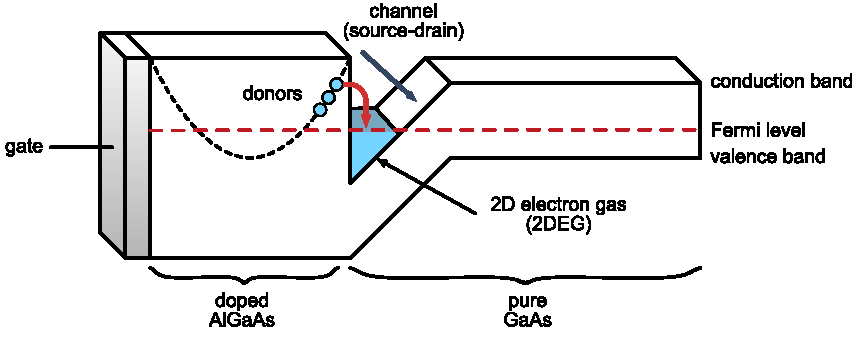
\includegraphics[scale=1]{./fig/HEMTBand.pdf}
\vspace{-0.5cm}
\caption{Bandstruktur eines typischen HEMT.
Elektronen aus dem stark n-dotierten AlGaAs diffundieren in das undotierte GaAs und bilden dort ein 2D-Elektronengas.
Über die Gatespannung wird die lage des Fermilevel und damit die menge and Elektronen im Leitungsband variiert.\cite{Thomas2016}}
\label{fig:HEMTBand}
\end{center}
\end{figure}

Bisherige niederfrequente kryogene Ausleseelektroniken basieren vorwiegend auf JFETs.
Die Technik von JEFTs stößt allerdings an zwei für diesen Anwendungsbereich entscheidende Grenzen.
Erstens frieren JFETs unter einer Temperatur von $\SI{100}{\kelvin}$ ein und werden idealer weise bei einer Temperatur von $\SI{130}{\kelvin}$ operiert.
Daher werden lange Kabel zwischen Ausleseelektronik und Detektor benötigt welche Auslesegeschwindigkeit und Signalqualität verringern.
Zweitens das minimal mögliche rauschen liegt in der Größenordnung von $\SI{1}{\nano\volt\per\sqrt\hertz}$ bei einer Frequenz von $\SI{1}{\kilo\hertz}$.
Das Funktionsprinzip von HEMTs und MOSFETs hingegen erlaubt es ihnen bei kryogenen Temperaturen operiert zu werden.
Diese Arten von Transistoren wurden bisher allerdings nicht verwendet aufgrund ihres hohen niederfrequenten $1/f$-Rauschen.

Infolge aktuelle Entwicklungen von Dr. Yong Jin an der Universität Paris-Süd ist es gelungen HEMTs zu entwerfen welche vielversprechende Eigenschaften aufweisen im Gegensatz zu handelsüblichen HEMTs.
Die Erste dieser Eigenschaften ist ein hervorragendes $1/f$-Rauschen von $\SI{0.46}{\nano\volt\per\sqrt\hertz}$ bei einer Frequenz von $\SI{1}{\kilo\hertz}$ und einer Temperatur von $\SI{4.2}{\kelvin}$.
Die Eingangskapazität liegt in der Größenordnung von $\SI{100}{\pico\farad}$ womit sie gut an die Detektorkapazität angepasst ist.
Zweitens liegt ihre benötigte Leistung in der Größenordnung von $\SI{30}{\mu\watt}$ deutlich unter der von JFET dadurch ist es möglich eine größere Anzahl von Ionisationskanälen im Kryostaten zu installieren.
Zuletzt sind diese HEMTs zur Anwendung bei kryogenen Temperaturen ausgelegt.
Werden JFETs verwendet ist es notwendig im Kryostaten eine Heizung einzubauen diese erzeugt Schhwarzkörperstrahlung welche wiederum vom Detektor absorbiert werden kann.
Außerdem muss sie von der Restlichen Anordnung isoliert werden. %TODO cite Membran
Die dazu verwendete Membran erzeugt zusätzliches niederfrequentes Rauschen durch ihre Schwingungen.\cite{HEMTYang2011, Jin2014}




